% THIS IS SIGPROC-SP.TEX - VERSION 3.1
% WORKS WITH V3.2SP OF ACM_PROC_ARTICLE-SP.CLS
% APRIL 2009
%
% It is an example file showing how to use the 'acm_proc_article-sp.cls' V3.2SP
% LaTeX2e document class file for Conference Proceedings submissions.
% ----------------------------------------------------------------------------------------------------------------
% This .tex file (and associated .cls V3.2SP) *DOES NOT* produce:
%       1) The Permission Statement
%       2) The Conference (location) Info information
%       3) The Copyright Line with ACM data
%       4) Page numbering
% ---------------------------------------------------------------------------------------------------------------
% It is an example which *does* use the .bib file (from which the .bbl file
% is produced).
% REMEMBER HOWEVER: After having produced the .bbl file,
% and prior to final submission,
% you need to 'insert'  your .bbl file into your source .tex file so as to provide
% ONE 'self-contained' source file.
%
% Questions regarding SIGS should be sent to
% Adrienne Griscti ---> griscti@acm.org
%
% Questions/suggestions regarding the guidelines, .tex and .cls files, etc. to
% Gerald Murray ---> murray@hq.acm.org
%
% For tracking purposes - this is V3.1SP - APRIL 2009

\documentclass{sig-alt-release2}
\special{papersize=8.5in,11in}
 \usepackage{url}
\usepackage{epsfig,endnotes}
%\usepackage{usenix,epsfig,endnotes}
%\usepackage{amsmath,amssymb,alltt,times,mathptmx,graphicx}
\usepackage{amsmath,amssymb,times,graphicx,amsfonts}
\usepackage{courier,subfigure,color,sped,url,wrapfig}
\usepackage{xspace}
\usepackage{balance}
\usepackage{enumitem}
%\usepackage[square,comma,numbers,sort&compress]{natbib} %REMOVED. this package setting comflict with 'sig-alternate-10pt.cls'
%\usepackage[font=sf, labelfont={sf,bf}, margin=0.5cm]{caption}
%\usepackage[labelfont={bf},margin=0.3cm]{caption}
%\usepackage{citesort}

% \usepackage[colorlinks=true, linkcolor=blue,
%               citecolor=blue, urlcolor=blue,
%               ps2pdf,                %%% hyper-references for ps2pdf
%               bookmarks=true,        %%% generate bookmarks ...
% 	      bookmarksopen=true,
%               bookmarksnumbered=true,%%% ... with numbers
%   ]{hyperref}

% \hypersetup{ pdfcreator  = {LaTeX with hyperref package},
%                pdfproducer = {dvips + ps2pdf} }
               
%\let\url\nolinkurl % because dvips cannot break url across lines
%\hypersetup{
%pdfauthor   = {},
%pdftitle    = {},
%pdfsubject  = {},
%pdfkeywords = {},
%}

\urlstyle{rm}

\usepackage{lastpage}

%%It seems these two packages must be loaded AFTER hyperref
\usepackage{algorithm}
\usepackage[noend]{algorithmic}
%\usepackage{enumitem}

%%% Local Variables:
%%% mode: latex
%%% TeX-master: "paper"
%%% End:

%\usepackage[T1]{fontenc}
%\usepackage[utf8]{inputenc}
% Useful macros for paper writing

\definecolor{brown}{cmyk}{0,0.81,1,0.60}
\definecolor{magenta}{rgb}{0.4,0.7,0}
\definecolor{gray}{rgb}{0.5,0.5,0.5}
\definecolor{red}{rgb}{1,0,0}
\definecolor{green}{rgb}{0.5,0,0.5}
\definecolor{blue}{rgb}{0,0,1}
\newcommand{\etc}{\emph{etc.}\xspace}
\newcommand{\ie}{\emph{i.e.,}\xspace}
\newcommand{\eg}{\emph{e.g.,}\xspace}
\newcommand{\etal}{\emph{et al.}\xspace}
\newcommand{\vlc}{vlc\xspace}
\newcommand{\SNOOZE}{Snooze\xspace}
\newcommand{\snz}{Snooze\xspace}
\newcommand{\POLICE}{Police\xspace}
\newcommand{\police}{Police\xspace}
\newcommand{\Police}{Police\xspace}
\newcommand{\PSTA}{Police Station\xspace}
\newcommand{\RTH}{\textbf{A}\xspace}
\newcommand{\ISI}{\textbf{B}\xspace}
%\newcommand{\reducefiguretopvmargin}{\vspace*{0ex}}
%\newcommand{\reducefigurebottomvmargin}{\vspace*{0.0ex}}
\newcommand{\reducefigurebottomvmarginsmall}{\vspace{-3mm}}
\newcommand{\reducefigurebottomvmargin}{\vspace{-4mm}}
\newcommand{\reducefigurecaptionmargin}{\vspace{-0mm}}
\newcommand{\reduceparavmargin}{\vspace*{0.0ex}}
%\newcommand{\reduceparavmargin}{\vspace*{-2.0ex}}
\newcommand{\reducesectionvmargin}{\vspace*{0.0ex}}
%\newcommand{\reducesectionvmargin}{\vspace*{-1.0ex}}
\newcommand{\reducevmarginsmall}{\vspace*{-.5ex}}
\newcommand{\reducevmarginone}{\vspace*{-1.0ex}}
\newcommand{\reducevmargintwo}{\vspace*{-2.0ex}}
\newcommand{\reducevmarginthree}{\vspace*{-3.0ex}}
\newcommand{\reducevmarginfour}{\vspace*{-4.0ex}}
\newcommand{\reducevmarginfive}{\vspace*{-5.0ex}}
\newcommand{\mypar}[1]{\vspace*{0.5ex}\noindent\textbf{#1}}
\newcommand{\mypari}[1]{\vspace*{0.5ex}\noindent\emph{#1}}

\newcommand{\spacesavecaption}[1]{\vspace*{0.0ex}\caption{#1}\vspace*{-3.5ex}}

\newcommand{\smallsection}[1]{\vspace*{1ex}\noindent\textbf{#1}}

% comment
\newcommand{\comment}[1]{{\color{gray}[\textsf{#1}]}}
\newcommand{\binliu}[1]{{\color{green}(KJ: #1)}}
\newcommand{\fei}[1]{{\color{red}(AS: #1)}}
\newcommand{\ramesh}[1]{{\color{blue}(RG: #1)}}
\newcommand{\yurong}[1]{{\color{brown}(SH: #1)}}
\newcommand{\camera}[1]{#1}

%\hyphenation{rate-allo-c-ation}

\newcommand{\equaref}[1]{Eq.~(\ref{eq:#1})}
\newcommand{\figref}[1]{\ref{fig:#1}}
\newcommand{\algref}[1]{Alg.~(\ref{alg:#1})}
\newcommand{\ruleref}[1]{\textsc{Rule}~\ref{rule:#1}}
\newtheorem{rul}{Rule}
\newcommand{\nonoverlapping}{\mbox{non-o}\-ver\-lap\-ping\xspace}
\newcommand{\interframe}{interframe\xspace}

\newcommand{\script}[1]{{{\cal{#1}}}}


\newtheorem{theorem}{Theorem}[section]
\newtheorem{lemma}[theorem]{Lemma}
\newtheorem{proposition}[theorem]{Proposition}
\newtheorem{corollary}[theorem]{Corollary}

% \newenvironment{definition}[1][Definition]{\begin{trivlist}
% \item[\hskip \labelsep {\bfseries #1}]}{\end{trivlist}}
% \newenvironment{example}[1][Example]{\begin{trivlist}
% \item[\hskip \labelsep {\bfseries #1}]}{\end{trivlist}}
% \newenvironment{remark}[1][Remark]{\begin{trivlist}
% \item[\hskip \labelsep {\bfseries #1}]}{\end{trivlist}}

\newcommand{\bm}[1]{\mbox{\boldmath{$#1$}}}
\newcommand{\ppcl}{Pickle\xspace}



%Figures

\newcommand{\scaleImage}[4]{
\begin{figure}[#1]
\centering
\includegraphics[width=#2\textwidth]{figs/#3}
\reducefigurecaptionmargin
\caption{#4\label{fig:#3}}
\reducefigurebottomvmarginsmall
\end{figure}
}

\newcommand{\scaleImageLabel}[5]{
\begin{figure}[#1]
\centering
\includegraphics[width=#2\textwidth]{figs/#3}
\reducefigurecaptionmargin
\caption{#4\label{fig:#5}}
\reducefigurebottomvmarginsmall
\end{figure}
}


\newcommand{\fullColumnFigs}[3]
{
\begin{figure*}[!tb]
  \centering
  {#1}
\reducefigurecaptionmargin
\caption{#2\label{fig:#3}}
\reducefigurebottomvmargin
\end{figure*}
}

\newcommand{\scaleTable}[4]{
\begin{table}[#1]
\centering
\includegraphics[width=#2\textwidth]{figs/#3}
\reducefigurecaptionmargin
\caption{#4\label{tbl:#3}}
\reducefigurebottomvmarginsmall
\end{table}
}

\newcommand{\oneColumnFigs}[3]
{
\begin{figure}[t]
  \centering
  {#1}
\reducefigurecaptionmargin
\caption{#2\label{fig:#3}}
\reducefigurebottomvmargin
\end{figure}
}

\newcommand{\subImage}[3]{% width, filename1, caption1, label1
    \hspace*{-2.0ex}
    \subfigure[#3]
    {
      \includegraphics[width=#1\textwidth]{figs/#2}
      \label{fig:#2}
    }
}

\newcommand{\subImagePadded}[5]{% figure_width, hpadding, filename1, caption1, label1
    \subfigure[#4]
    {
      \hspace{#2\textwidth}
      \includegraphics[width=#1\textwidth]{figs/#3}
      \hspace{#2\textwidth}
      \label{fig:#5}
    }
}

\newcommand{\subImageWithNoLable}[2]{% width, filename1, caption1, label1
      \includegraphics[width=#1\textwidth]{figs/#2}
}

%%% Local Variables: 
%%% mode: latex
%%% TeX-master: "paper"
%%% End: 

\newcommand{\jyr}[1]{{\color{red}#1}}
%\newcommand{MediaScope}{MediaScope\xspace}
\newcommand{\mscope}{MediaScope\xspace}
\newcommand{\crs}{Credit Reward Scheme\xspace}
\begin{document}
\conferenceinfo{IPSN'13,} {April 8--11, 2013, Philadelphia, Pennsylvania, USA.}
\CopyrightYear{2013}
\crdata{978-1-4503-1959-1/13/04}
\clubpenalty=10000
\widowpenalty = 10000

\title{Demo Abstract - MediaScope: Selective On-Demand Media Retrieval from Mobile Devices\titlenote{\scriptsize Research was sponsored by the Army Research Laboratory and was
accomplished under Cooperative Agreement Number W911NF-09-2-0053.  The
views and conclusions contained in this document are those of the
authors and should not be interpreted as representing the official
policies, either expressed or implied, of the Army Research Laboratory
or the U.S. Government.  The U.S. Government is authorized to
reproduce and distribute reprints for Government purposes
notwithstanding any copyright notation here on.}}

%\subtitle{[Extended Abstract]
%\titlenote{A full version of this paper is available as
%\textit{Author's Guide to Preparing ACM SIG Proceedings Using
%\LaTeX$2_\epsilon$\ and BibTeX} at
%\texttt{www.acm.org/eaddress.htm}}}
%
% You need the command \numberofauthors to handle the 'placement
% and alignment' of the authors beneath the title.
%
% For aesthetic reasons, we recommend 'three authors at a time'
% i.e. three 'name/affiliation blocks' be placed beneath the title.
%
% NOTE: You are NOT restricted in how many 'rows' of
% "name/affiliations" may appear. We just ask that you restrict
% the number of 'columns' to three.
%
% Because of the available 'opening page real-estate'
% we ask you to refrain from putting more than six authors
% (two rows with three columns) beneath the article title.
% More than six makes the first-page appear very cluttered indeed.
%
% Use the \alignauthor commands to handle the names
% and affiliations for an 'aesthetic maximum' of six authors.
% Add names, affiliations, addresses for
% the seventh etc. author(s) as the argument for the
% \additionalauthors command.
% These 'additional authors' will be output/set for you
% without further effort on your part as the last section in
% the body of your article BEFORE References or any Appendices.

\numberofauthors{6} %  in this sample file, there are a *total*
% of EIGHT authors. SIX appear on the 'first-page' (for formatting
% reasons) and the remaining two appear in the \additionalauthors section.
%
\author{
% You can go ahead and credit any number of authors here,
% e.g. one 'row of three' or two rows (consisting of one row of three
% and a second row of one, two or three).
%
% The command \alignauthor (no curly braces needed) should
% precede each author name, affiliation/snail-mail address and
% e-mail address. Additionally, tag each line of
% affiliation/address with \affaddr, and tag the
% e-mail address with \email.
%
% 1st. author
\alignauthor
Xing Xu\titlenote{\scriptsize The first two authors contributed equally to this work and their names are listed alphabetically by first name.}\\
       \affaddr{University of Southern California}\\
       \email{xingx@usc.edu}
\alignauthor
Yurong Jiang \\
  \affaddr{University of Southern California} \\
  \email{yurongji@usc.edu}
\alignauthor
Peter Terlecky \\
       \affaddr{City University of New York}\\
       \email{pterlecky@gc.cuny.edu}
\and
\alignauthor
Tarek Abdelzaher \\
       \affaddr{University of Illinois at Urbana-Champaign}\\
       \email{zaher@illinois.edu}
\alignauthor
Amotz Bar-Noy\\
       \affaddr{City University of New York}\\
       \email{amotz@sci.brooklyn.cuny.edu}
\alignauthor
Ramesh Govindan\\
       \affaddr{University of Southern California}\\
       \email{ramesh@usc.edu}
}
% There's nothing stopping you putting the seventh, eighth, etc.
% author on the opening page (as the 'third row') but we ask,
% for aesthetic reasons that you place these 'additional authors'
% in the \additional authors block, viz.
% Just remember to make sure that the TOTAL number of authors
% is the number that will appear on the first page PLUS the
% number that will appear in the \additionalauthors section.

\maketitle
\begin{abstract}
Motivated by an availability gap for visual media, where images and
videos are uploaded from mobile devices well after they are generated,
we explore the \emph{selective,
  timely retrieval} of media content from a collection of mobile
devices.
%
We envision this capability being driven by \emph{similarity-based
  queries} posed to a cloud search front-end, which in turn
dynamically retrieves media objects from mobile devices that best
match the respective queries within a given time limit.
%
Building upon a crowd-sensing framework, we have designed and
implemented a system called \mscope that provides this capability.
%
\mscope is an extensible framework that supports nearest-neighbor
and other geometric queries on the feature space (e.g., clusters,
spanners), and contains novel retrieval algorithms that attempt to
maximize the retrieval of relevant information.
%
From experiments on a prototype, \mscope is shown to achieve
near-optimal query completeness and low to moderate overhead on mobile
devices.
\end{abstract}

\vspace{-0.2cm}
\category{H.3.3}{Information Storage and Retrieval}{Information Search and Retrieval}
\category{H.3.4}{Information Storage and Retrieval}{Systems and Software}
\category{H.4.0}{Information Systems Applications}{General}
\category{C.2.4}{Computer-Communication Networks}{Distributed Systems}

\vspace{-0.2cm}
\terms{Design, Experimentation, Performance}
\vspace{-0.2cm}
\keywords{Crowd-sensing, Image-Retrieval, Feature-Extraction, Mobile-Device} % NOT required for Proceedings
\
\

\section{Introduction}

Cameras on mobile devices have given rise to significant
\emph{sharing} of media data (photos and videos).
%
Users upload visual media to online social networks like
Facebook~\cite{facebook}, as well as to dedicated sharing sites like
Flickr~\cite{flickr} and Instagram~\cite{instagram}.
%
However, these uploads are often not \emph{immediate}.
%
Camera sensors on mobile devices have been increasing in both image
and video resolution far faster than cellular network capacity.
%
Moreover, in response to growing demand and consequent
contention for wireless spectrum, cellular data providers have
imposed data usage limits, which disincentivize immediate photo
uploading and create an \emph{availability gap} (the time between a photo or image is taken and it is uploaded).
%
This availability gap can be on the order of several days.

\camera{If media data was available immediately, it might enable
  scenarios where there is a need for recent (or fresh) information.}
%
Consider the following scenario: users at a mall or some other
location take pictures and video of some event (e.g. an accident or
altercation).
%
An investigative team that wants visual evidence of the event
%shepherd review
%, and
could have searched or browsed images on
%shepherd review
%, say, of
a photo sharing service such as Flickr
%shepherd review
%, and may have been able
to retrieve evidence in a timely fashion.
%shepherd review
% in the absence of an availability gap.
%
%shepherd review
%\camera{In this example, because there is an availability gap, the
%team may not have access to fresher information than it otherwise
%might have.}
%

% This has resulted in an \emph{availability gap}: media is shared/uploaded
% often much later than the data is generated.  But in some situation,
% people might be more interested in some more  realtime update from
% their friends, or get some information of a special event known by
% their friends, but current social network can't guarantee that since
% social network only provides us a somewhat passive information
% broadcast way. Thus we need a system that would keep those who are
% interested in up-to-date wlling-to-share content and eliminate the
% \emph{freshness} gap.

To bridge this availability gap, and to enable this and other missed
opportunities,
%shepherd review
% (Section~\ref{sec-2}),
 we consider a novel
%shepherd review
%(Section~\ref{sec-5})
capability for
%shepherd review
% selective and timely
 on-demand retrieval of images from mobile devices.
%
Specifically, we develop a system called \mscope that permits
concurrent
%shepherd review
%timely
geometric queries in feature space on
%shepherd review
%media data
that may be distributed across several mobile devices.
%shepherd review
%\mscope is an extensible framework that supports different kinds of
%queries (Section~\ref{sec-3}).
%
%\mscope queries permit nearest-neighbor searches on image feature
%spaces, \emph{spanners} that retrieve samples of images that span
%the feature space, or \emph{cluster representatives} that are samples
%of clusters in the feature space.
%

%\emph{timeliness}, \camera{which is defined as the query response time duration after issued, may be quite critical in some scenario%(e.g. military settings). In other cases, timeliness can ensure service
%  interactivity (in much the same way as service level agreements on
%  latency in Web services ensure low user-perceived delay), which can
%  be a crucial differentiator for search.}

\camera{
%However,
Wireless bandwidth is limited and can vary, \emph{concurrent
  queries} might compete for limited bandwidth, and query results can
be large (since images are large and many images can match a query).
%
These factors can result in unacceptably long query response times,
which can impede usability.
%
In some cases, applications might need lower query response times for
correctness; in the scenario above, time may be of the
essence in taking action (e.g., apprehending suspects).
%
%shepherd review
%So we impose a \emph{timeliness constraint} on query completion; thus,
%the central challenge in the design of \mscope is to retrieve query
%results, in the presence of \emph{concurrent queries}, while
%respecting the \camera{each queries'} timeliness constraints.
%
}

\mscope addresses this challenge using an approach that trades off
query completeness\footnote{Completeness is intuitively defined as the proportion of desired images uploaded before the timeliness bound.}, while meeting
timeliness requirements
%shepherd review
\camera{(measured by the time between the issue of the query and when a query result is returned)}.
%
It incorporates a novel credit-assignment scheme that is used to
%shepherd review
%differentially
weight queries as well as differentiate query results
by their ``importance''.
%
A novel credit and timeliness-aware scheduling algorithm that also
adapts to wireless bandwidth variability ensures that query completeness
%shepherd review
%(measured by the total credit of all the returned results of the query)
is optimized.
%
A second important challenge is to enable accurate yet
computationally-feasible feature extraction.
%
\mscope addresses this challenge by finding sweet spots in the
trade-off between accuracy and computational cost, for extracting
features from images and frames from videos.


% The general idea is, today's smart phone with good computational
% capability can generate a small metadata for each media object(videos
% and photos), aggregate them and upload metadata to our cloud server
% when the network is available.
% %
% Then our cloud server only stores these metadata , whenever there is a
% query, based on the query type and parameters, our cloud server
% figures out what are the best media objects(photos or video clips) to
% answer the query and ask the corresponding phones to upload such
% selected objects.
%

\vspace{-0.3cm}
\section{MediaScope Design}
MediaScope is a system that supports timely similarity-based
queries on media objects stored on mobile devices.
%
Mediascope is conceptually partitioned across a cloud component
called MSCloud, and another component called MSMobile that runs
on mobile devices.
%
This partitioned design leverages the computation and storage
power of clouds to support geometric queries on the feature space;
mobile devices provide sensing and storage for media objects.

These components interact as follows
(Figure~\ref{fig:architecture}).
%
In the background, whenever participants take photos or videos,
the \emph{Feature Extractor} component of MSMobile continuously
extracts image and video features and uploads them to the
\emph{MSCloudDB}.
%
Users (e.g., a security officer or a reporter) pose queries to
MSCloud using a standard web interface, possibly on a mobile
device.
%
These queries are processed by the \emph{MSCloudQ} query
processing engine, which uses the features stored in the MSCloudDB
to compute the query results.
%
The results of the queries identify the media objects that need to
be retrieved from individual mobile devices.
%
In some cases, a media object may already have been retrieved as a
result of an earlier query; query results are also \emph{cached}
in MSCloudDB in order to optimize retrieval.
%
MSCloudQ coordinates with an \emph{Object Uploader} component on
MSMobile in order to retrieve query results.

MediaScope uses a publicly available crowd sensing platform called
Medusa~\cite{Medusa}, to enable programmed interaction between
MSCloud and Medusa, and to support MediaScope's timeliness
requirement, we made several modifications to Medusa Platform.
%
The most challenging component of MediaScope is support for
concurrent queries, we designed a \emph{credit assignment
mechanism}, the main idea is as follows, each query is awarded a
certain amount of credit, and the query itself is responsible for
assigned these amount of credit to the qualified objects given by
the query optimizer, so each object of uploading request in
MSMobile is associated with a credit, MSMobile is going to upload
in a way that maximizing the total credit of uploadable objects.
%
Our current instantiation of MediaScope supports three
qualitatively different queries: nearest neighbor, clusters, and
spanners. Detailed implementation is discussed in the full paper.

\begin{figure}
\centering 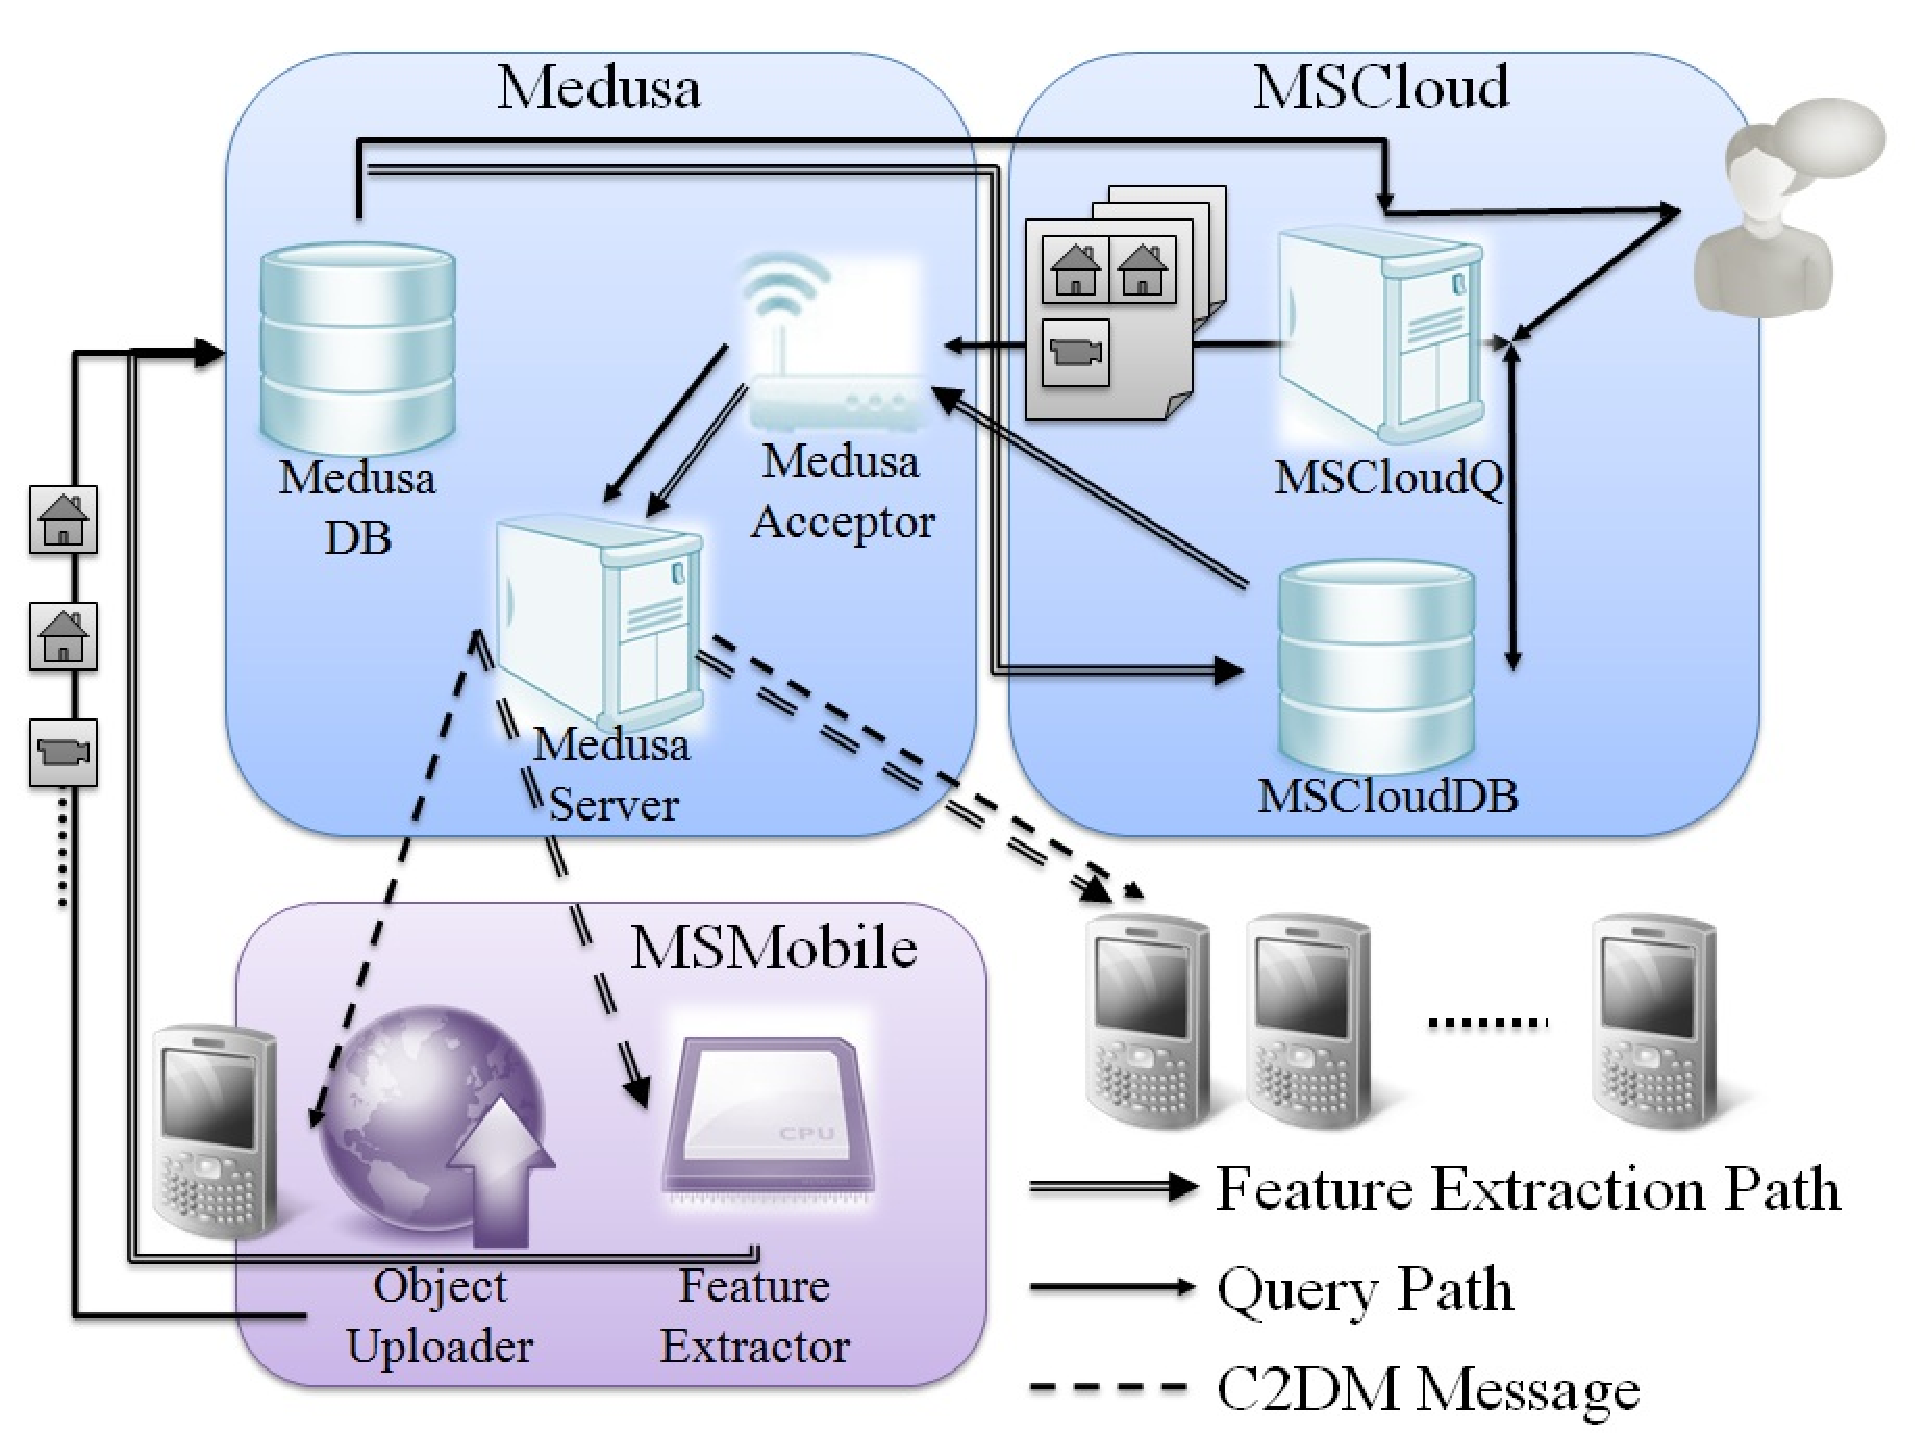
\epsfig{file=pics/architecture.eps, width=2.3in} \caption{System Architecture Work Flow}
\label{fig:architecture}
\vspace{-0.6cm}
\end{figure}

\begin{figure}
\centering 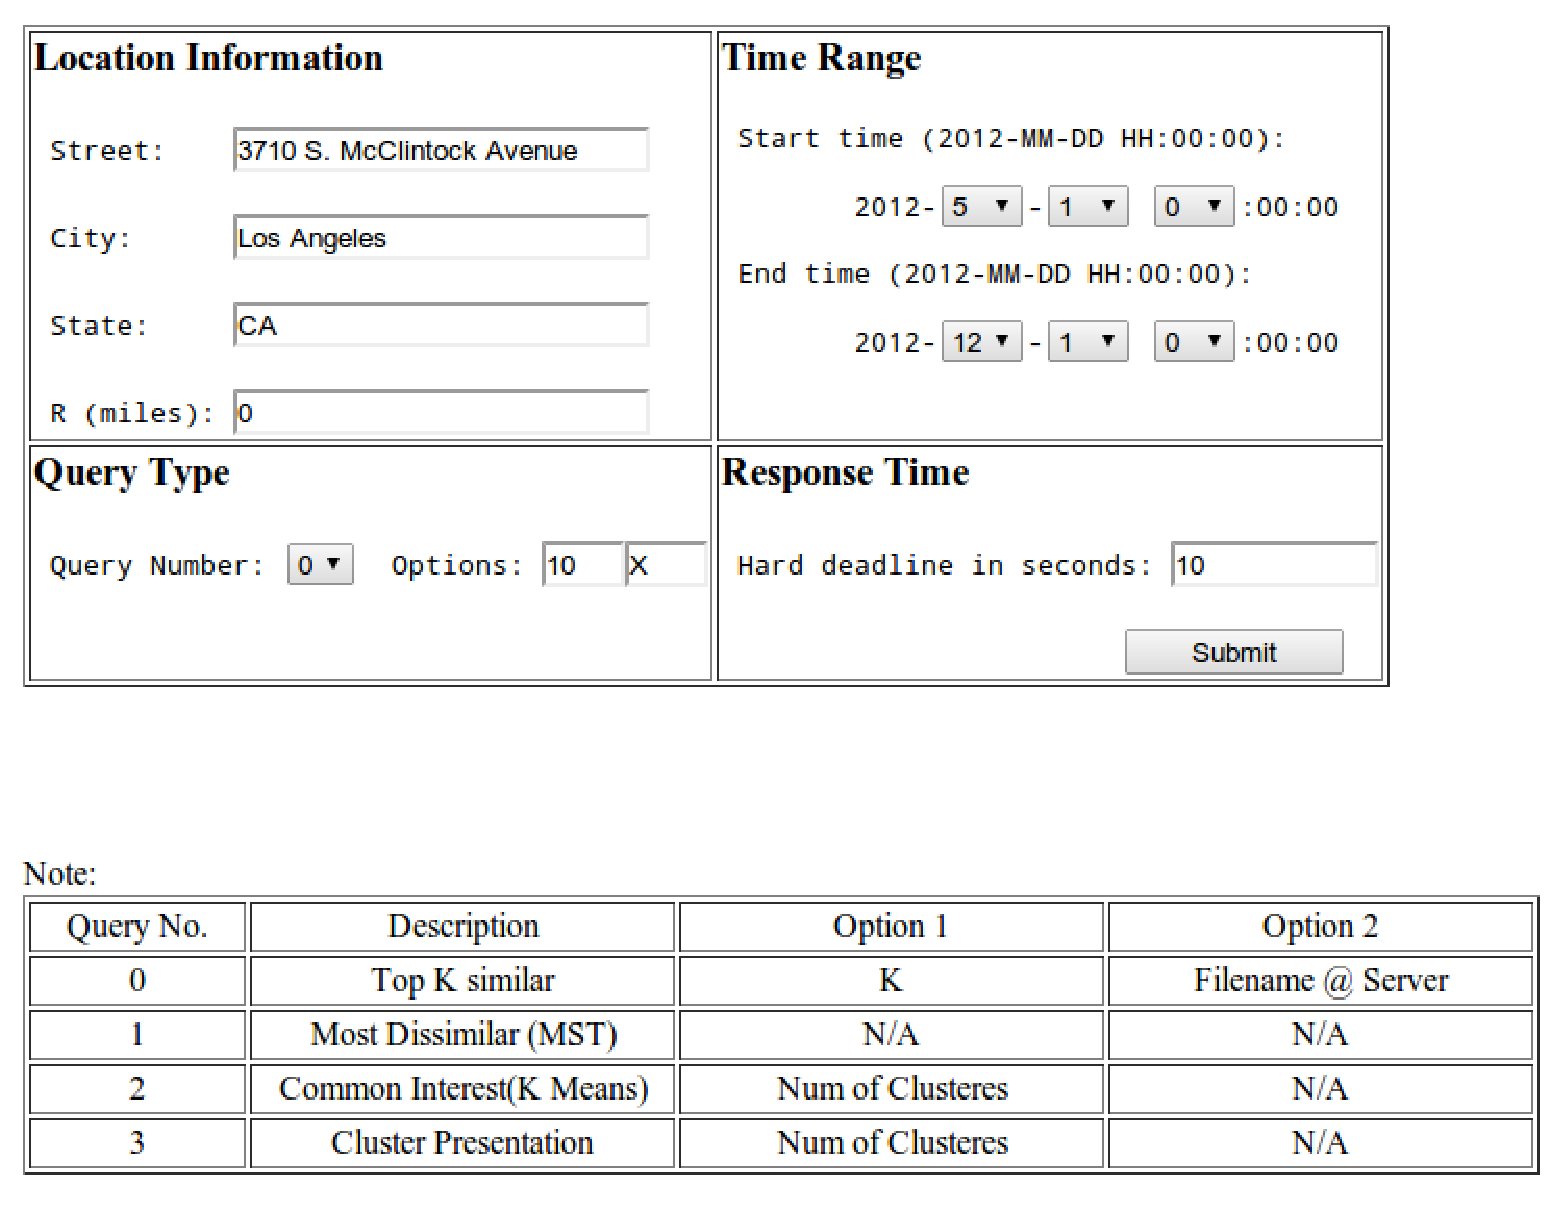
\epsfig{file=pics/queryinterface.eps, width=2.3in} \caption{Query Interface} \label{fig:interface}
\vspace{-0.8cm}
\end{figure}
\vspace{-0.3cm}
\section{Demo Details}
We have built MediaScope prototype system using a commodity server
machine and Android smartphones. The query interface of MSCloudQ
is shown in Figure~\ref{fig:interface}. This demonstration will
show the crucial steps of MediaScope: 1) the mobile device once
capture an image, the corresponding feature will be extracted and
uploaded to MSCloudDB automatically; 2) when MSCloud received
query, it will select best media files and ask for uploading; 3)
MSMobile will upload media files selected by MSCloud, and then
MSCloud return results. For step 2), it is possible that MSCloud
get concurrent queries (in the demo, we will issue multiple
queries from different tabs of the browser); consequently,
MSMobile will receive concurrent uploading tasks, sometimes this
means that not all the uploading tasks can be completely uploaded
before its timeliness bound and in this situation, the scheduling
is critical for the sake of maximizing information (credit)
collected.
\vspace{-0.3cm}
\section{Related Work}
There are some other works focus on search over resources,
\cite{sensorranking} deal with people-centric sensor data; however
MediaScope focuses on image search. MediaScope is inspired by leveraging
semantics of features \cite{crowdsearch,photonet}, techniques for
content-based image retrieval from a centralized database of
images \cite{faceted,imgseek} and image retrieval from
mobile devices \cite{content1,content2}. Compared to
existing works, MediaScope uniquely supports searches on a cloud
server, but where the content is stored on the mobile devices and
is retrieved on demand.

%
% The following two commands are all you need in the
% initial runs of your .tex file to
% produce the bibliography for the citations in your paper.
\vspace{-0.3cm}
\bibliographystyle{abbrv}
\small{\small{\bibliography{sigproc}}}  % sigproc.bib is the name of the Bibliography in this case
% You must have a proper ".bib" file
%  and remember to run:
% latex bibtex latex latex
% to resolve all references
%
% ACM needs 'a single self-contained file'!
%
%APPENDICES are optional
%\balancecolumns

% That's all folks!
\end{document}
